\section{CipherStore: System Overview and Application Model}
\label{sec:cipherstore-overview}

CipherStore turns storage-resident records into LWE ciphertexts through a programmable CSD path. Record selection and projection precede encryption, so the number of generated ciphertexts follows the data required by the application. This section presents the system organization, the application-level task contract, and the mapping from a task to device execution.

\subsection{System Overview}
\label{subsec:cipherstore-organization}

Figure~\ref{fig:cipherstore-overview} shows the generation path. A client on the Host accepts a task describing stored records and the desired encrypted values. The SoC--FPGA CSD combines an SSD, device-side shared-memory namespaces (SLMs), and FPGA operators for selection, projection, and LWE encryption. The client configures these operators through the CSD interface, retrieves the generated ciphertexts, and can supply them to an FHE computation back end.

\begin{figure*}[t]
  \centering
  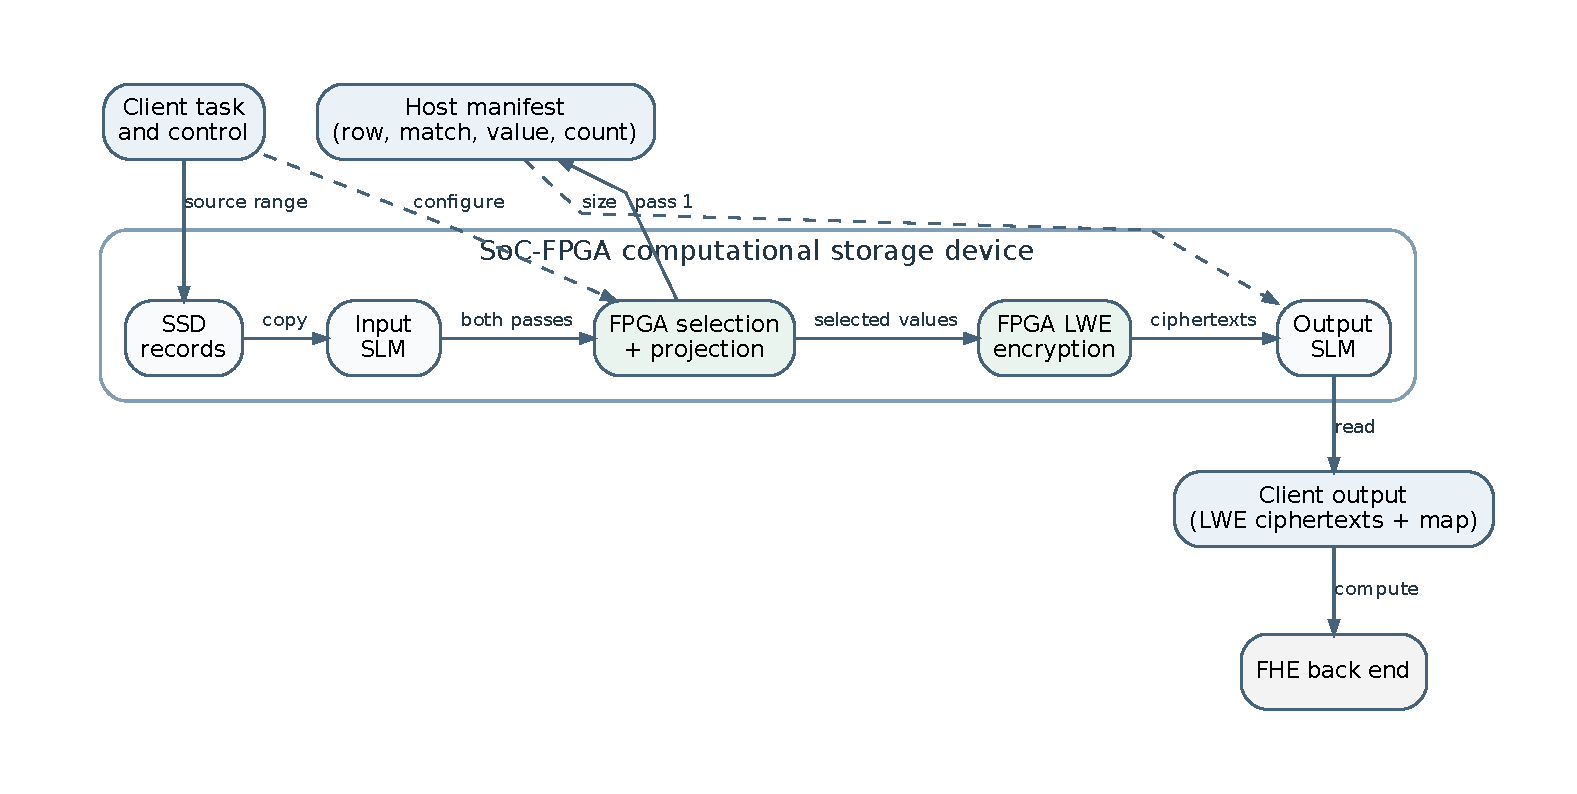
\includegraphics[width=0.94\textwidth]{../figures/system_overview.pdf}
  \Description{A client task selects records on a computational storage device. SSD records enter an input SLM. The FPGA filter returns a selection manifest in a discovery pass, then sends selected values to an LWE encryption operator in a second pass. Ciphertexts leave through an output SLM for client and optional FHE back-end use.}
  \caption{CipherStore generation path. The CSD copies source records into an input SLM, discovers the selected rows, and streams selected values through FPGA LWE encryption into an output SLM. Solid arrows carry data or selection results; dashed arrows represent client configuration and output sizing.}
  \label{fig:cipherstore-overview}
\end{figure*}

The Host manages task submission, operator contexts, and result delivery. It loads the secret key into the encryption context, while the CSD performs record selection and ciphertext generation. The discovery result returns row identities and selected projected values to the client; the subsequent generation pass emits LWE ciphertexts. The client retains the row mapping alongside the ciphertext sequence so that downstream results can be associated with their source records.

\subsection{Application Model}
\label{subsec:task-model}

CipherStore represents each request as $T=(D,Q,E,O)$: source data $D$, query $Q$, encryption configuration $E$, and output action $O$. Table~\ref{tab:cipherstore-task} maps these fields to the CSD path. The source is identified by an SSD namespace and logical block range, with a fixed-record schema defining field types and byte offsets. The query uses these fields to determine which records contribute values to encryption.

\begin{table}[H]
  \centering
  \small
  \setlength{\tabcolsep}{4pt}
  \caption{Application task fields and their execution mapping.}
  \label{tab:cipherstore-task}
  \begin{tabular}{@{}p{0.24\columnwidth}p{0.66\columnwidth}@{}}
    \toprule
    Field & Application declaration and CSD action \\
    \midrule
    Data $D$ & SSD namespace and range, record count, width, and schema; copied to the input SLM. \\
    Query $Q$ & Predicate and projected field; compiled into FPGA filter configuration. \\
    Encryption $E$ & TFHE parameter preset and key reference; configure LWE ciphertext generation. \\
    Result $O$ & Ordered ciphertexts and source-row mapping; delivered to the client or a computation back end. \\
    \midrule
    Runtime profile & Device endpoints, batch size, and transfer settings; control execution without changing task semantics. \\
    \bottomrule
  \end{tabular}
\end{table}

For records $r_0,\ldots,r_{N-1}$, let $P_Q(r_i)$ be the predicate and $\pi_Q(r_i)$ the projected value specified by $Q$. The task produces
\begin{equation}
\mathcal{C}_T=
\bigl(\operatorname{Enc}_{E}(\pi_Q(r_i))\bigr)_{i\in\mathcal{I}_Q},
\quad
\mathcal{I}_Q=(i\mid P_Q(r_i)=\mathrm{true}),
\label{eq:ciphertext-generation-task}
\end{equation}
with indices in source-record order. The companion mapping $\mathcal{I}_Q$ identifies the source record of each ciphertext after filtering. In the TFHE instantiation used here, the projected value is an unsigned byte encoded as four two-bit LWE ciphertext blocks, as described in Section~\ref{subsec:lwe-background}. Predicate evaluation can use the integer fields specified by the record schema.

The task specifies which values become ciphertexts; a separate runtime profile selects batch and transport parameters. The client validates the task and divides its source range into LBA-aligned batches. A global record offset attached to each batch preserves the mapping between generated ciphertexts and source records across the complete task.

\subsection{Mapping Tasks to Device Execution}
\label{subsec:cipherstore-execution}

For each batch, the client copies the corresponding SSD blocks into an input SLM. It then invokes the FPGA filter in discovery mode. This pass produces a deterministic-size manifest with one 64-byte entry per record and a 64-byte summary. Each entry reports its row index and match result; for a matched row it also carries the projected value. The Host obtains the selected count from the device-generated summary and uses it to configure the ciphertext output range.

The client next runs a filter--encryption program on the same input SLM. The filter streams the selected values directly to the LWE encryption operator, which writes the resulting ciphertexts to an output SLM. Thus, selection controls both the amount of cryptographic work and the size of the ciphertext result. The Host reads the output and associates its ordered ciphertexts with the row mapping from discovery. If a batch selects no records, no encryption program is issued.

The application can consume the generated LWE ciphertexts directly or pass them to a homomorphic-computation back end. In the latter workflow, returned ciphertext results can be decrypted by the CSD and applied to the selected source-row positions. Generation and downstream computation are connected by the same ciphertext sequence and row mapping defined in Equation~\eqref{eq:ciphertext-generation-task}.
